\documentclass[10pt,t]{beamer}

\usepackage{ 
academicons,
adjustbox, 
    amsmath,
    amssymb,
    apacite,
   beamerthemesplit,
   bm,  
    booktabs,
    breqn,
    catchfilebetweentags,
    color,
    colortbl,
    csquotes,
   % enumitem,
    epigraph,
    fancyvrb,
    fontawesome,
    graphicx,
    hyperref,
    pifont,
    scalerel,
    soul,
    tabularx,
    tikz,
    xcolor,
    xfrac}
    

    
    %\usepackage[TU]{fontenc}
%\usepackage{}
    
% Colors
\definecolor{RadiantOrchid}{rgb}{0.678431 0.349020 1.000000}
\definecolor{RoyalBlue}{rgb}{0.141176 0.301961 1.000000}
\definecolor{Aluminum}{rgb}{0.611765 0.588235 0.533333}
\definecolor{MistedYellow}{rgb}{0.909804 0.831373 0.301961}
\definecolor{Sangria}{rgb}{0.603922 0.000000 0.525490}
\definecolor{MauveMist}{rgb}{0.800000 0.678431 0.929412}
\definecolor{Cognac}{rgb}{0.466667 0.356863 0.407843}
\definecolor{BrightCobalt}{rgb}{0.098039 0.513725 0.894118}
\definecolor{Cypress}{rgb}{0.266667 0.392157 0.211765}
\definecolor{SeaFog}{rgb}{0.631373 0.650980 0.780392}
\definecolor{DriedHerb}{rgb}{0.517647 0.498039 0.364706}
\definecolor{DesertSage}{rgb}{0.639216 0.674510 0.600000}
\definecolor{StormyWeather}{rgb}{0.345098 0.392157 0.427451}
\definecolor{OakBuff}{rgb}{0.815686 0.615686 0.364706}
\definecolor{BiscayBay}{rgb}{0.035294 0.474510 0.533333}
\definecolor{ReflectingPond}{rgb}{0.125490 0.243137 0.290196}
\definecolor{CadmiumOrange}{rgb}{0.976471 0.580392 0.443137}
\definecolor{CashmereRose}{rgb}{0.807843 0.529412 0.623529}
\definecolor{AmethystOrchid}{rgb}{0.572549 0.415686 0.650980}
\definecolor{Riverside}{rgb}{0.298039 0.415686 0.572549}
\definecolor{Sharkskin}{rgb}{0.513725 0.517647 0.529412}
\definecolor{AiryBlue}{rgb}{0.572549 0.713725 0.835294}
\definecolor{AuroraRed}{rgb}{0.725490 0.227451 0.196078}
\definecolor{WarmTaupe}{rgb}{0.686275 0.580392 0.513725}
\definecolor{DustyCedar}{rgb}{0.678431 0.364706 0.364706}
\definecolor{LushMeadow}{rgb}{0.000000 0.431373 0.317647}
\definecolor{SpicyMustard}{rgb}{0.847059 0.682353 0.278431}
\definecolor{PottersClay}{rgb}{0.619608 0.274510 0.141176}
\definecolor{Bodacious}{rgb}{0.717647 0.419608 0.639216}
\definecolor{PlacidBlue}{rgb}{0.529412 0.831373 0.980392}
\definecolor{VioletTulip}{rgb}{0.560784 0.611765 1.000000}
\definecolor{Hemlock}{rgb}{0.611765 0.960784 0.650980}
\definecolor{Paloma}{rgb}{0.650980 0.760784 0.729412}
\definecolor{Sand}{rgb}{0.800000 0.729412 0.521569}
\definecolor{Freesia}{rgb}{1.000000 0.858824 0.000000}
\definecolor{Cayenne}{rgb}{0.941176 0.258824 0.439216}
\definecolor{CelosiaOrange}{rgb}{1.000000 0.368627 0.200000}
\definecolor{DazzlingBlue}{rgb}{0.078431 0.431373 1.000000}
\definecolor{PurpleHaze}{rgb}{0.439216 0.490196 0.850980}
\definecolor{Comfrey}{rgb}{0.235294 0.647059 0.333333}
\definecolor{MagentaPurple}{rgb}{0.458824 0.145098 0.388235}
\definecolor{Aquamarine}{rgb}{0.615686 0.776471 0.847059}
\definecolor{Scuba}{rgb}{0.000000 0.698039 0.792157}
\definecolor{LuciteGreen}{rgb}{0.490196 0.811765 0.713725}
\definecolor{ClassicBlue}{rgb}{0.113725 0.305882 0.537255}
\definecolor{ToastedAlmond}{rgb}{0.823529 0.698039 0.603922}
\definecolor{StrawberryIce}{rgb}{0.890196 0.525490 0.560784}
\definecolor{Tangerine}{rgb}{0.968627 0.572549 0.337255}
\definecolor{Custard}{rgb}{0.917647 0.850980 0.545098}
\definecolor{Marsala}{rgb}{0.584314 0.321569 0.317647}
\definecolor{GlacierGray}{rgb}{0.776471 0.796078 0.800000}
\definecolor{DuskBlue}{rgb}{0.490196 0.631373 0.749020}
\definecolor{Treetop}{rgb}{0.305882 0.431373 0.219608}
\definecolor{Woodbine}{rgb}{0.498039 0.501961 0.250980}
\definecolor{Sandstone}{rgb}{0.780392 0.552941 0.419608}
\definecolor{Titanium}{rgb}{0.541176 0.521569 0.529412}
\definecolor{LavenderHerb}{rgb}{0.701961 0.560784 0.694118}
\definecolor{RoseQuartz}{rgb}{0.968627 0.792157 0.788235}
\definecolor{PeachEcho}{rgb}{0.968627 0.470588 0.419608}
\definecolor{Serenity}{rgb}{0.568627 0.658824 0.815686}
\definecolor{SnorkelBlue}{rgb}{0.011765 0.309804 0.517647}
\definecolor{Buttercup}{rgb}{0.980392 0.878431 0.235294}
\definecolor{LimpetShell}{rgb}{0.596078 0.866667 0.870588}
\definecolor{LilacGray}{rgb}{0.596078 0.588235 0.643137}
\definecolor{Fiesta}{rgb}{0.866667 0.254902 0.196078}
\definecolor{IcedCoffee}{rgb}{0.694118 0.560784 0.415686}
\definecolor{GreenFlash}{rgb}{0.474510 0.780392 0.325490}
\definecolor{PrimroseYellow}{rgb}{0.964706 0.819608 0.333333}
\definecolor{PaleDogwood}{rgb}{0.929412 0.803922 0.760784}
\definecolor{Hazelnut}{rgb}{0.811765 0.690196 0.584314}
\definecolor{IslandParadise}{rgb}{0.584314 0.870588 0.890196}
\definecolor{Greenery}{rgb}{0.533333 0.690196 0.294118}
\definecolor{Flame}{rgb}{0.949020 0.333333 0.172549}
\definecolor{PinkYarrow}{rgb}{0.807843 0.192157 0.458824}
\definecolor{Niagara}{rgb}{0.329412 0.517647 0.643137}
\definecolor{Kale}{rgb}{0.352941 0.447059 0.278431}
\definecolor{LapisBlue}{rgb}{0.000000 0.294118 0.552941}


    
% Theme modifications
\usetheme[progressbar=foot]{metropolis}
\addtobeamertemplate{frametitle}{}{\vspace{1em}}
\renewcommand{\emph}[1]{{{\color{bordeaux}#1}}}
\renewcommand\bibliographytypesize{\footnotesize}


\setbeamercolor{block title}{use=structure,fg=black,bg=black!15!white}
\setbeamercolor{block body}{use=structure,fg=black,bg=black!10!white}

\setbeamercolor{background canvas}{bg=white}
%\setbeamercolor{normal text}{fg=black}

\renewcommand\bibliographytypesize{\footnotesize}

%\setlist[enumerate]{label=\bf\alph*)}

% Super lazy shorthands
\newcommand{\e}[1]{\emph{#1}}
\newcommand{\strng}[1]{{{\color{jade}#1}}}

\newcommand{\bi}{\begin{itemize}}
\newcommand{\ei}{\end{itemize}}
\renewcommand{\i}{\item[$\bullet$]}
\renewcommand{\j}{\item[-]}

\newcommand{\bc}{\begin{columns}}
\newcommand{\ec}{\end{columns}}
\renewcommand{\c}[2]{{\color{#1}\texttt{#2}}}

\newcommand{\ex}[1]{\begin{block}{#1}\vspace{0pt}}
\newcommand{\xe}{\end{block}\vspace{3ex}}

\newcommand{\beq}{\begin{eqnarray*}}
\newcommand{\eeq}{\end{eqnarray*}}

\renewcommand{\c}[2]{{\color{#1}\texttt{#2}}}

\newcommand{\code}[1]{\texttt{#1}}


% Font
\usefonttheme[onlymath]{serif}

% Unusual symbols
\newcommand{\cmark}{\ding{51}}% Check mark
\newcommand{\xmark}{\ding{55}}% Cross mark
\let\lightning\faBolt % Lightning bolt


% Colors
\definecolor{amber}{rgb} {0.99, 0.75, 0.20}
\definecolor{violet}{rgb}{0.55, 0.20, 0.90}
\definecolor{jade}{rgb}  {0.00, 0.66, 0.42}
\definecolor{blue}{rgb}  {0.00, 0.39, 0.64}
\definecolor{gold}{rgb}  {1.00, 0.82, 0.00}
\definecolor{lightgrey}{rgb}  {0.85, 0.85, 0.85}
\definecolor{offwhite}{rgb}   {0.965, 0.965, 0.965}
\definecolor{paleyellow}{rgb} {1, .975, 0.85}
\definecolor{bordeaux}{rgb}   {0.50, 0.10, 0.10}
\definecolor{royalblue}{rgb}  {0.26, 0.41, 0.88}
\definecolor{darkgreen}{rgb}  {0.10, 0.50, 0.10}

\definecolor{titleCiteAColor}{rgb} {0.5, 0.7, 0.85}
\definecolor{titleCiteColor}{rgb}  {0.5, 0.7, 0.85}


% Hyperlink colors
\hypersetup{
    citecolor=,  % Clear global citecolor, see below
    colorlinks=true,
    linkcolor=blue,
    filecolor=magenta,      
    urlcolor=cyan,
}


% Extend cite for color
%\let\plainCiteA\citeA
%\renewcommand{\citeA}[2][gray]{{\color{#1}\plainCiteA{#2}}}
%\let\plainCite\cite
%\renewcommand{\cite}[2][gray]{{\color{#1}\plainCite{#2}}}
%
%\newcommand{\titleCiteA}[1]{\citeA[titleCiteAColor]{#1}}
%\newcommand{\titleCite}[1]{\cite[titleCiteColor]{#1}}


% Math and logic notation
\newcommand{\given}{{ \mid }}

\newcommand{\lxor}{\veebar}
\renewcommand{\l}[1]{\mbox{ \sc{#1} }}

\renewcommand{\therefore}{\Rightarrow}
\renewcommand{\implies}{\rightarrow}
\newcommand{\equivalent}{\leftrightarrow}
\newcommand{\nonequivalent}{\not\leftrightarrow}


% Graphics
\usepackage{graphicx}
%\graphicspath{ {p/} }
\usepackage{tikz}
\usetikzlibrary{tikzmark}

% Title page defaults
\author[shortname]{Michael D. Lee}
\institute{University of California Irvine\\(Singapore Management University)\\(Adelaide University)}
\date{}

\setbeamercolor{block title}{use=structure,fg=black,bg=black!15!white}
\setbeamercolor{block body}{use=structure,fg=black,bg=black!10!white}

%\setbeamertemplate{itemize items}[circle]
\usepackage{adjustbox}
\usepackage[formats]{listings}

% Add your keywords here, and have this in a separate file
% and include it in your preamble
\lstset{
  language=R,
  basicstyle=\ttfamily\small,
  keywordstyle=\color{blue},
  morekeywords={dunif, dinterval, dbin, phi, dbern}
}

%\lstdefinestyle{mystyle}{
%    backgroundcolor=\color{backcolour},   
%    commentstyle=\color{codegreen},
%    keywordstyle=\color{magenta},
%    numberstyle=\tiny\color{codegray},
%    stringstyle=\color{codepurple},
%    basicstyle=\ttfamily\footnotesize,
%    breakatwhitespace=false,         
%    breaklines=true,                 
%    captionpos=b,                    
%    keepspaces=true,                 
%    numbers=left,                    
%    numbersep=5pt,                  
%    showspaces=false,                
%    showstringspaces=false,
%    showtabs=false,                  
%    tabsize=2
%}
%
%\lstset{style=mystyle}




\title{Cognitive Models, Wisdom of the Crowd, Citizen Science, and Frogs: An Extension of \protect\shortciteA{brown2024cognitive}}


\begin{document}

\maketitle

\begin{frame}[fragile]{Detecting Frogs}
\vspace{-1em}
\bi
\i Citizen scientists listen to audio recording clips trying to detect the presence of various ground and tree frogs by their calls
\ei
\begin{center}
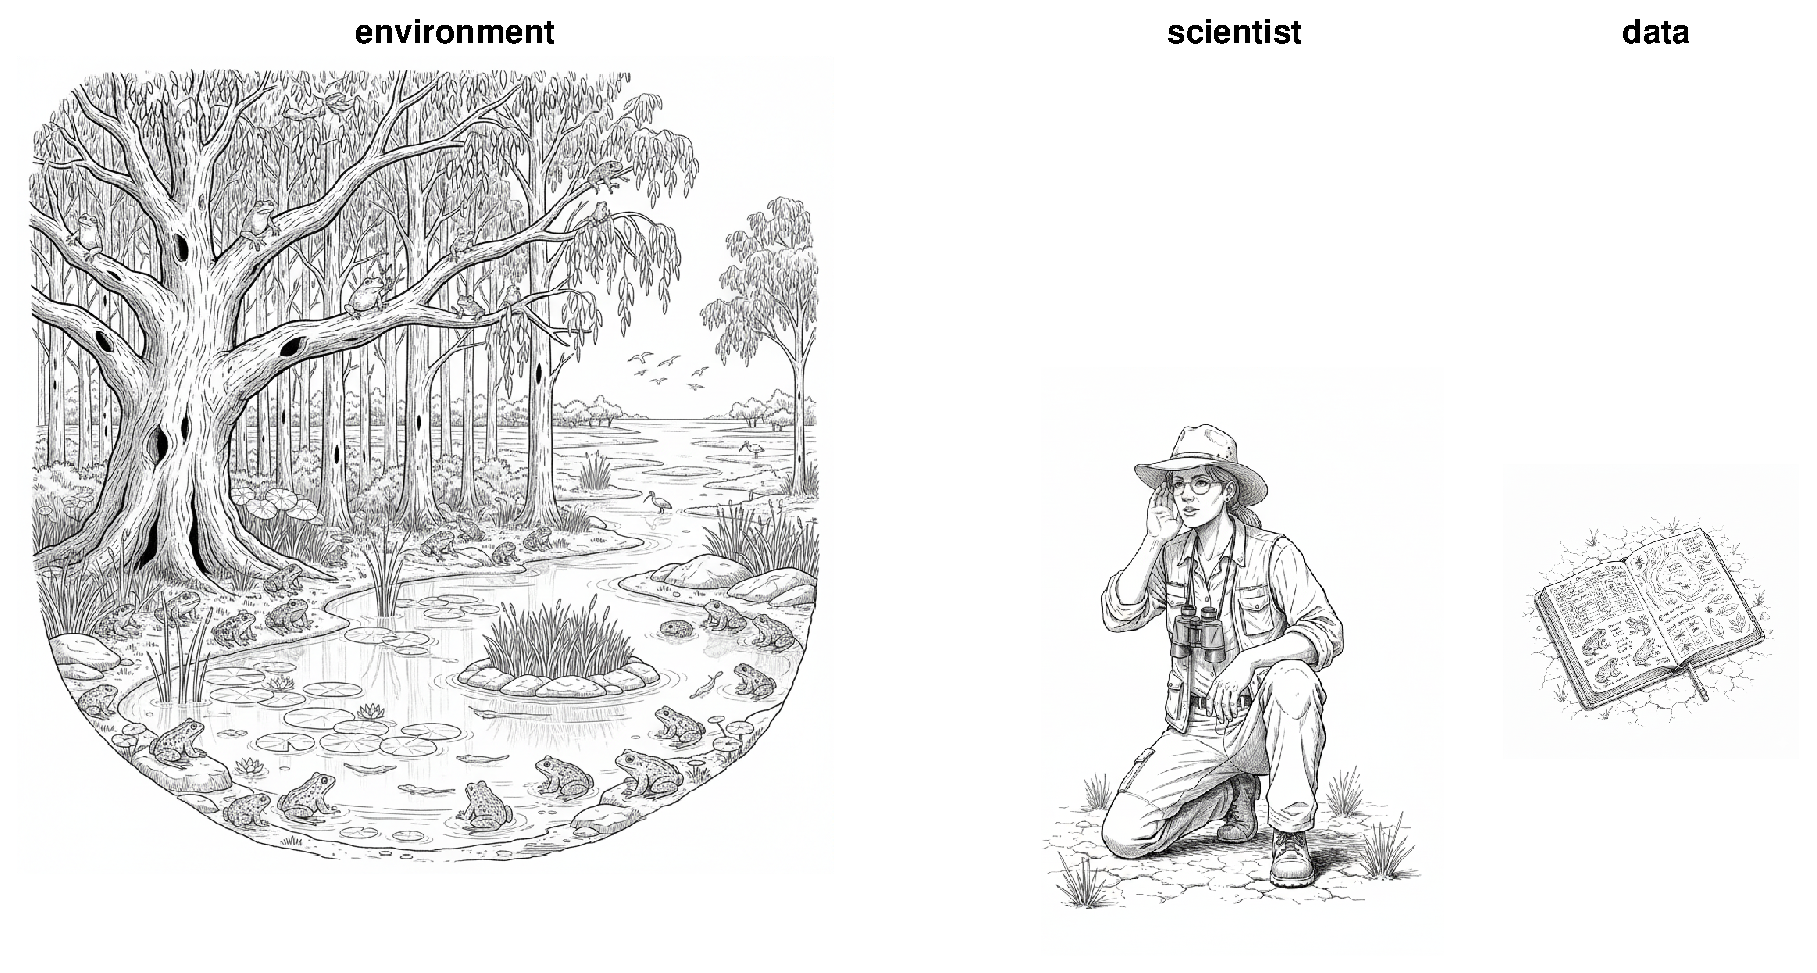
\includegraphics[width = \columnwidth, trim = {0cm 0cm 0cm 0cm}, clip]{../analyses/figures/frogPond_0.eps}\\
\end{center}
\end{frame}

\begin{frame}[fragile]{Detecting Frogs}
\vspace{-1em}
\bi
\i Multiple citizen scientists can independently listen to the same clip
\vspace{1em}
\ei
\begin{center}
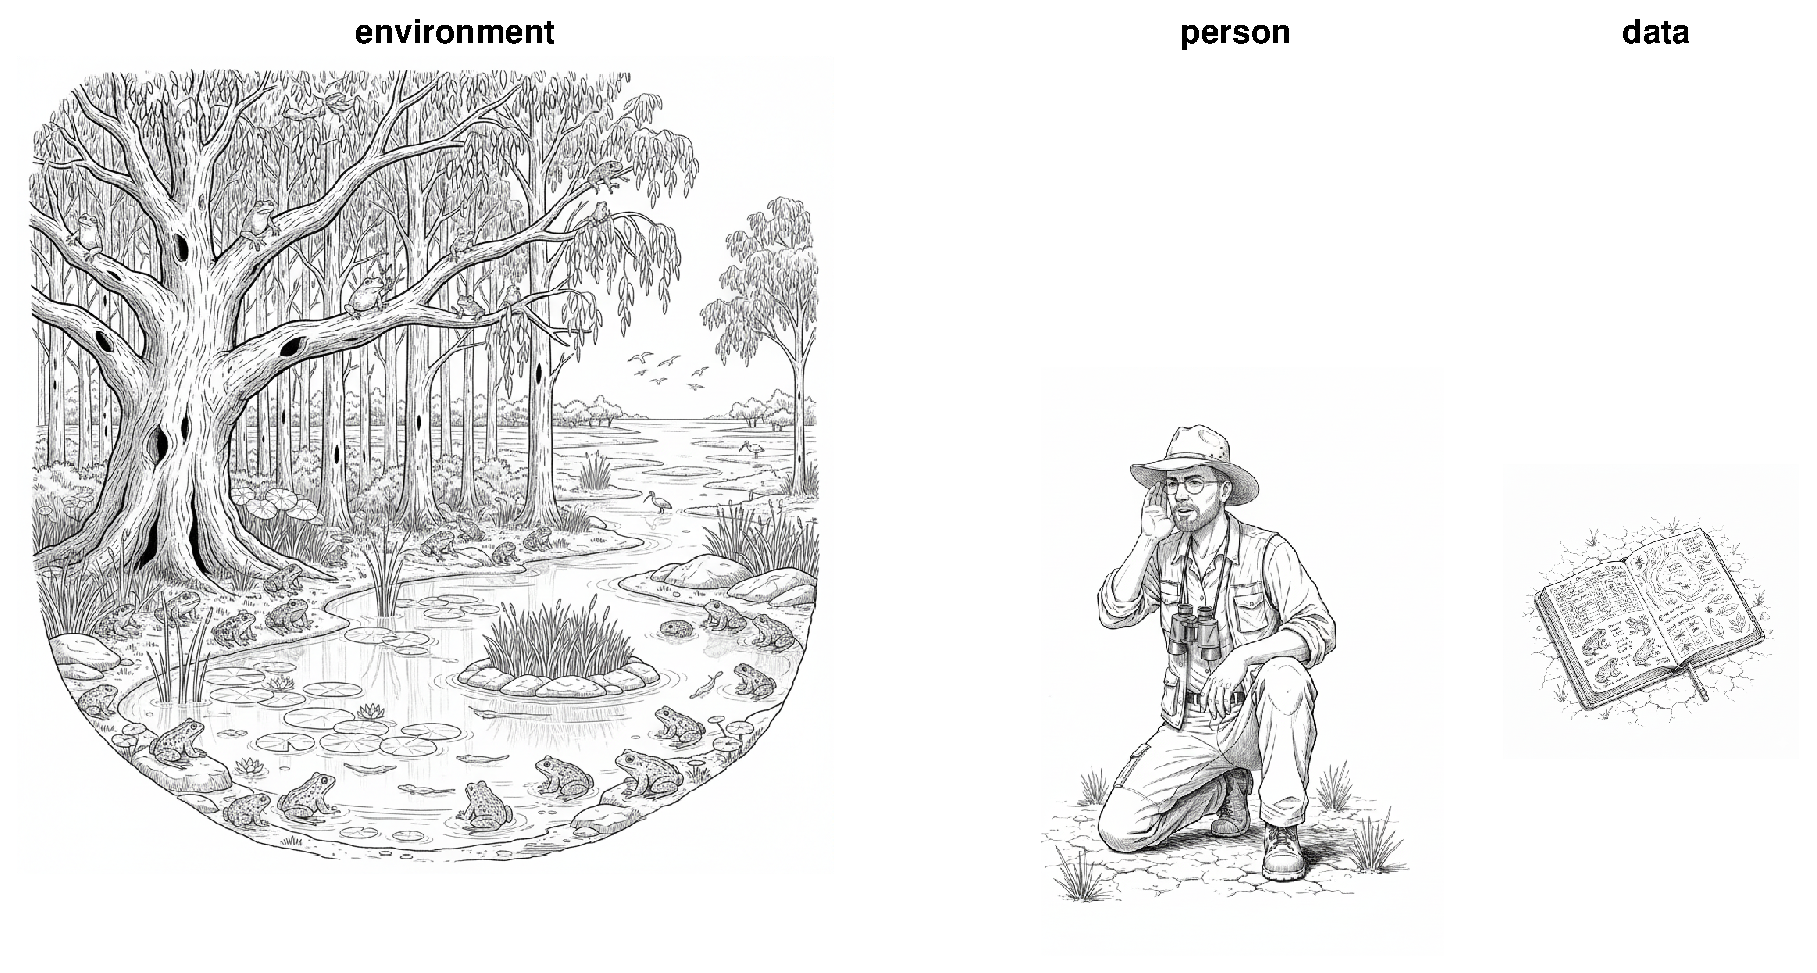
\includegraphics[width = \columnwidth, trim = {0cm 0cm 0cm 0cm}, clip]{../analyses/figures/frogPondMale.eps}\\
\end{center}
\end{frame}

\begin{frame}[fragile]{Detecting Frogs}
\vspace{-1em}
\bi
\i The same citizen scientist can listen to multiple clips
\vspace{1em}
\ei
\begin{center}
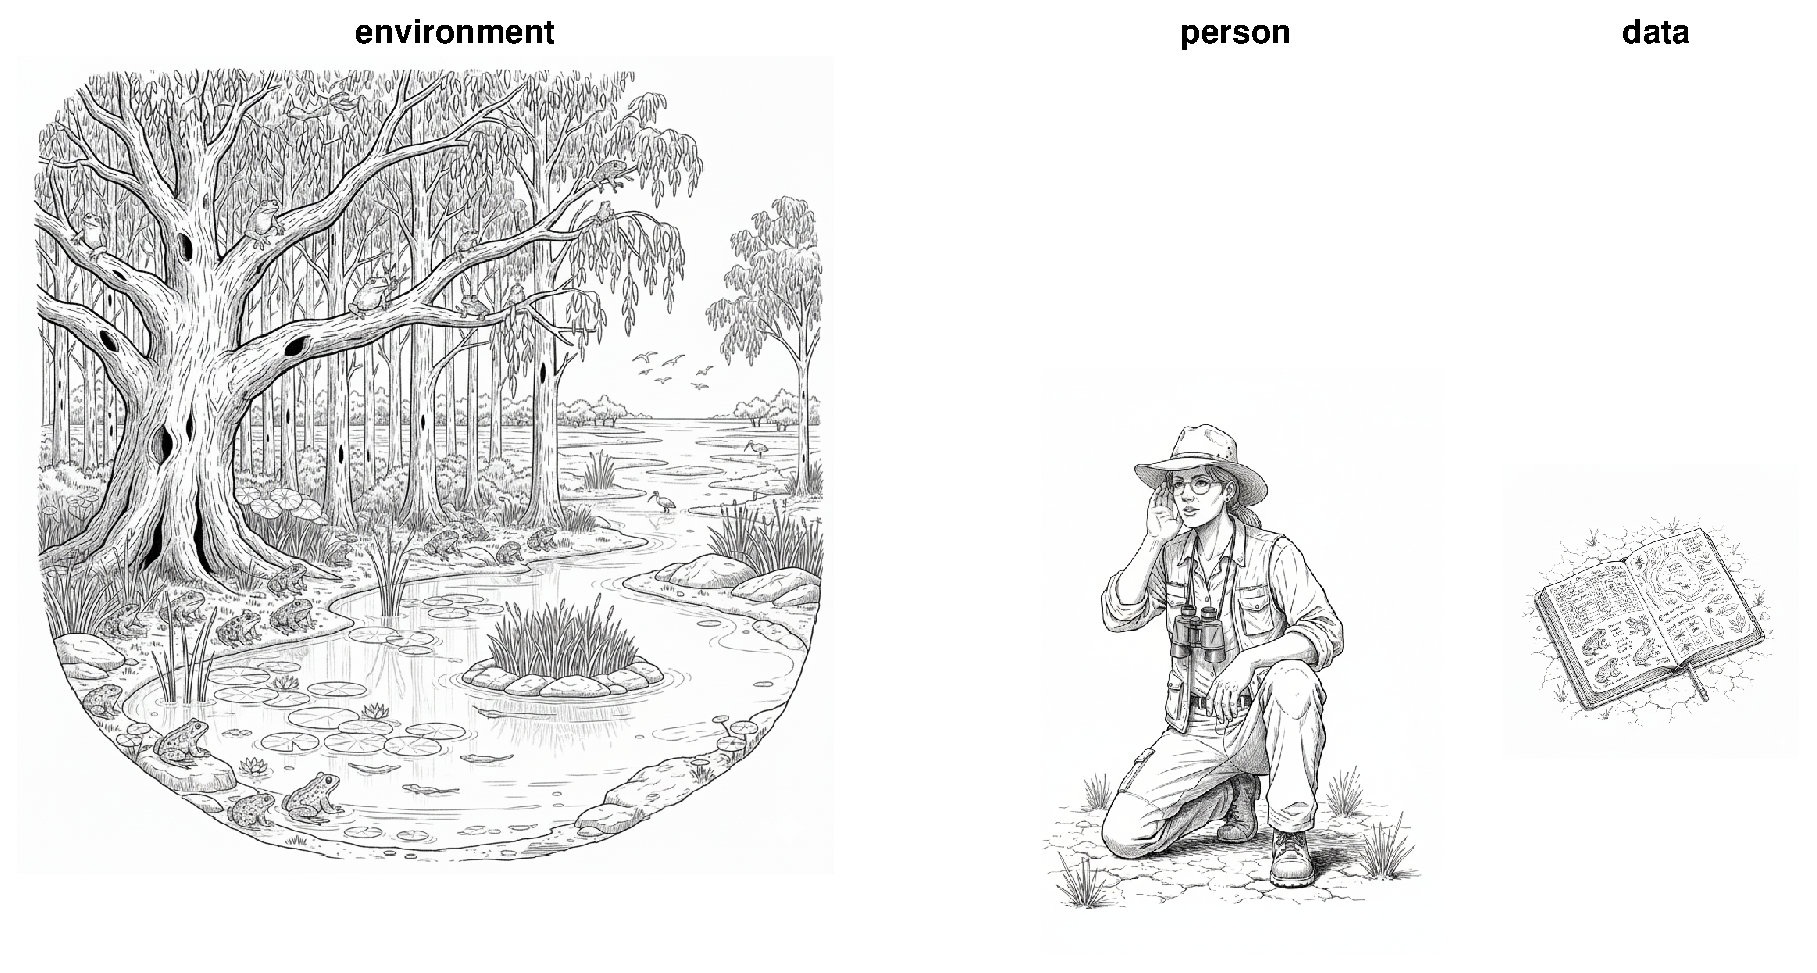
\includegraphics[width = \columnwidth, trim = {0cm 0cm 0cm 0cm}, clip]{../analyses/figures/frogPondZonderKikker.eps}\\
\end{center}
\end{frame}

\begin{frame}[fragile]{Data}
\vspace{-1em}
\bi
\i The joint and marginal distributions of people judging clips shows
\bi 
\j lots of people judge few clips, but a few people judge many
\j the data collection system aims to have five judgments for each frog in each clip
\ei
\vspace{0em}
\ei
\begin{center}
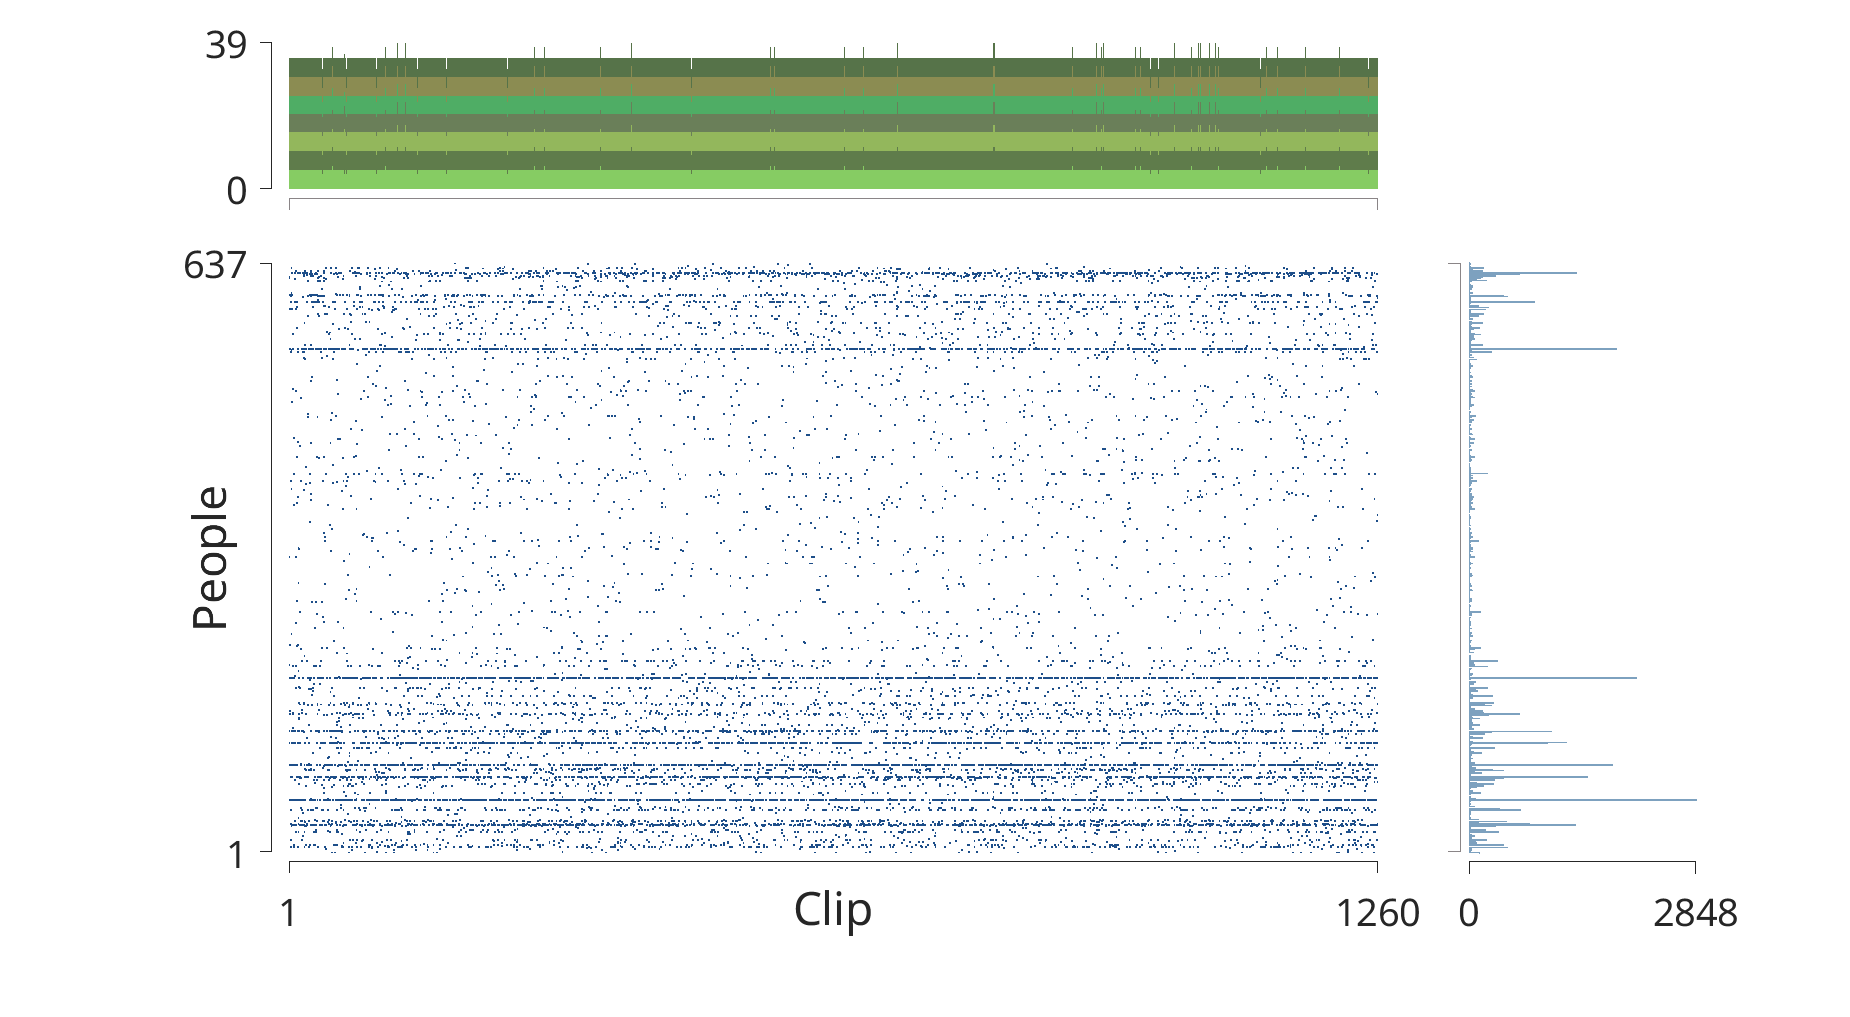
\includegraphics[width = \columnwidth, trim = {0cm 0cm 0cm 0cm}, clip]{../analyses/figures/peopleByClip.eps}\\
\end{center}
\end{frame}


\begin{frame}[fragile]{Crowd Proportions and the Truth}
\vspace{-1em}
\bi
\i The blue marks indicate the ground truth (expert derived) presence of each type of frog across the sequence of clips
\i The yellow bars show the proportion of citizen scientists who judged a frog was present in each clip
\vspace{1em}
\ei
\begin{center}
\includegraphics[width = \columnwidth, trim = {0cm 0cm 0cm 0cm}, clip]{../analyses/figures/voteCrowd.eps}\\
\end{center}
\end{frame}

\begin{frame}[fragile]{Crowd Performance}
\vspace{-2em}
\bi
\i ROC curves show reasonable wisdom the crowd performance for five of the frog types
\bi
\j the BMTF and GSF tree frogs are not well detected
\j both are rarely present but people produce many false alarms
\ei
\ei
\begin{center}
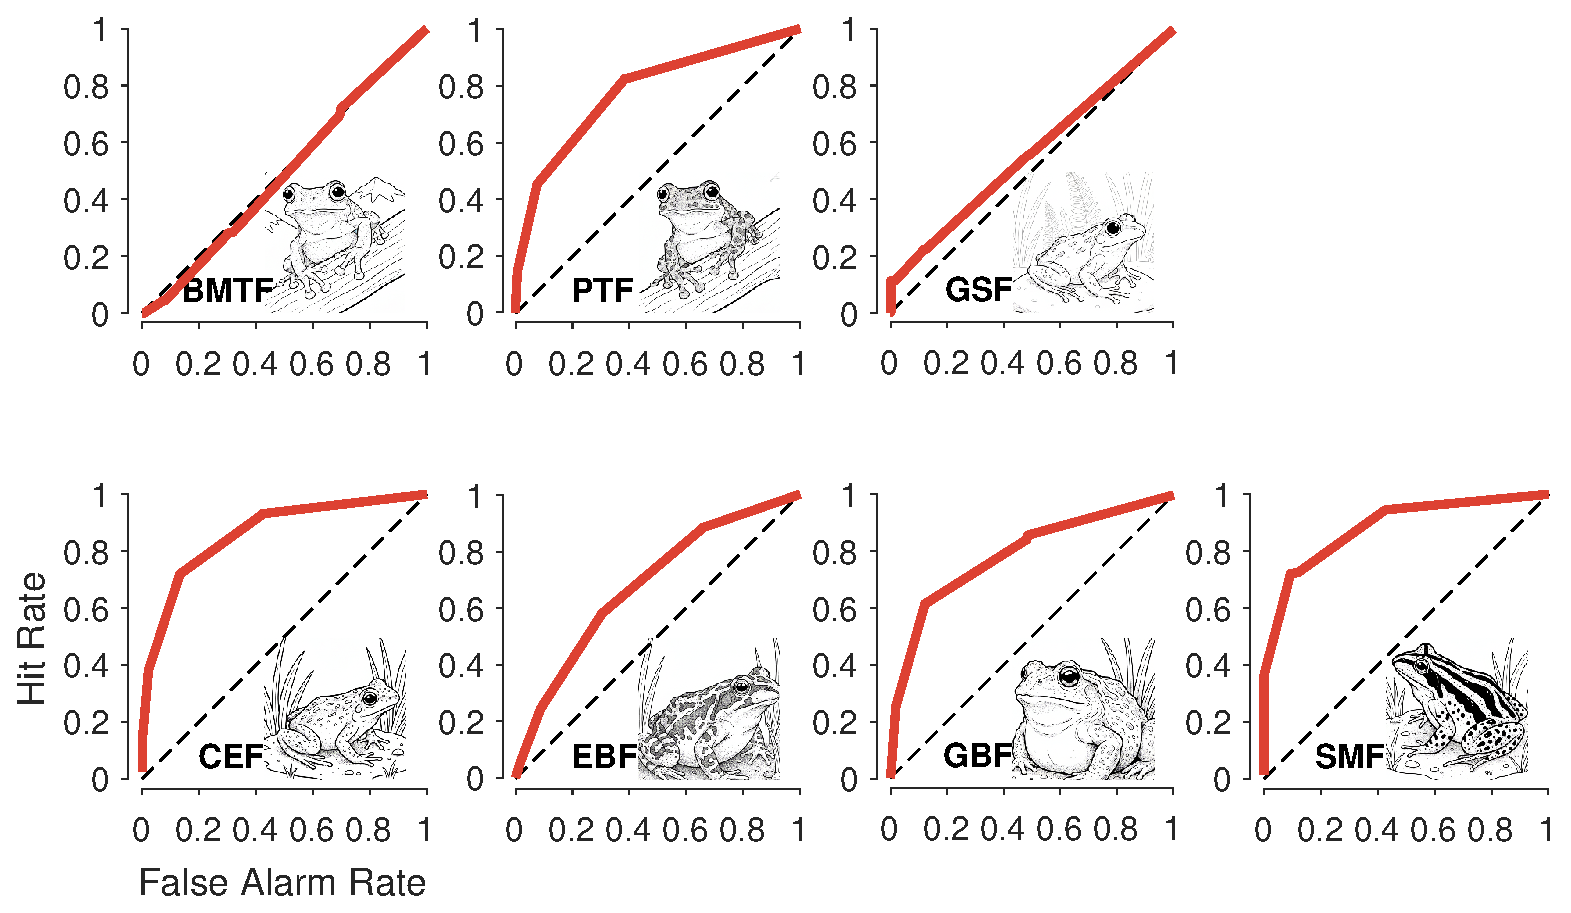
\includegraphics[width = \columnwidth, trim = {0cm 0cm 0cm 0cm}, clip]{../analyses/figures/voteROCs.eps}\\
\end{center}
\end{frame}

\begin{frame}[fragile]{Model-Based Wisdom of the Crowd}
\vspace{-1em}
\bi
\i The model-based approach uses cognitive models to explain how the behavior data were produced \shortcite{brown2024cognitive, lee2024using}
\bi
\j make inferences about the cognitive abilities and biases of individuals
\j make inferences about latent states of nature
\ei
\ei
\begin{center}
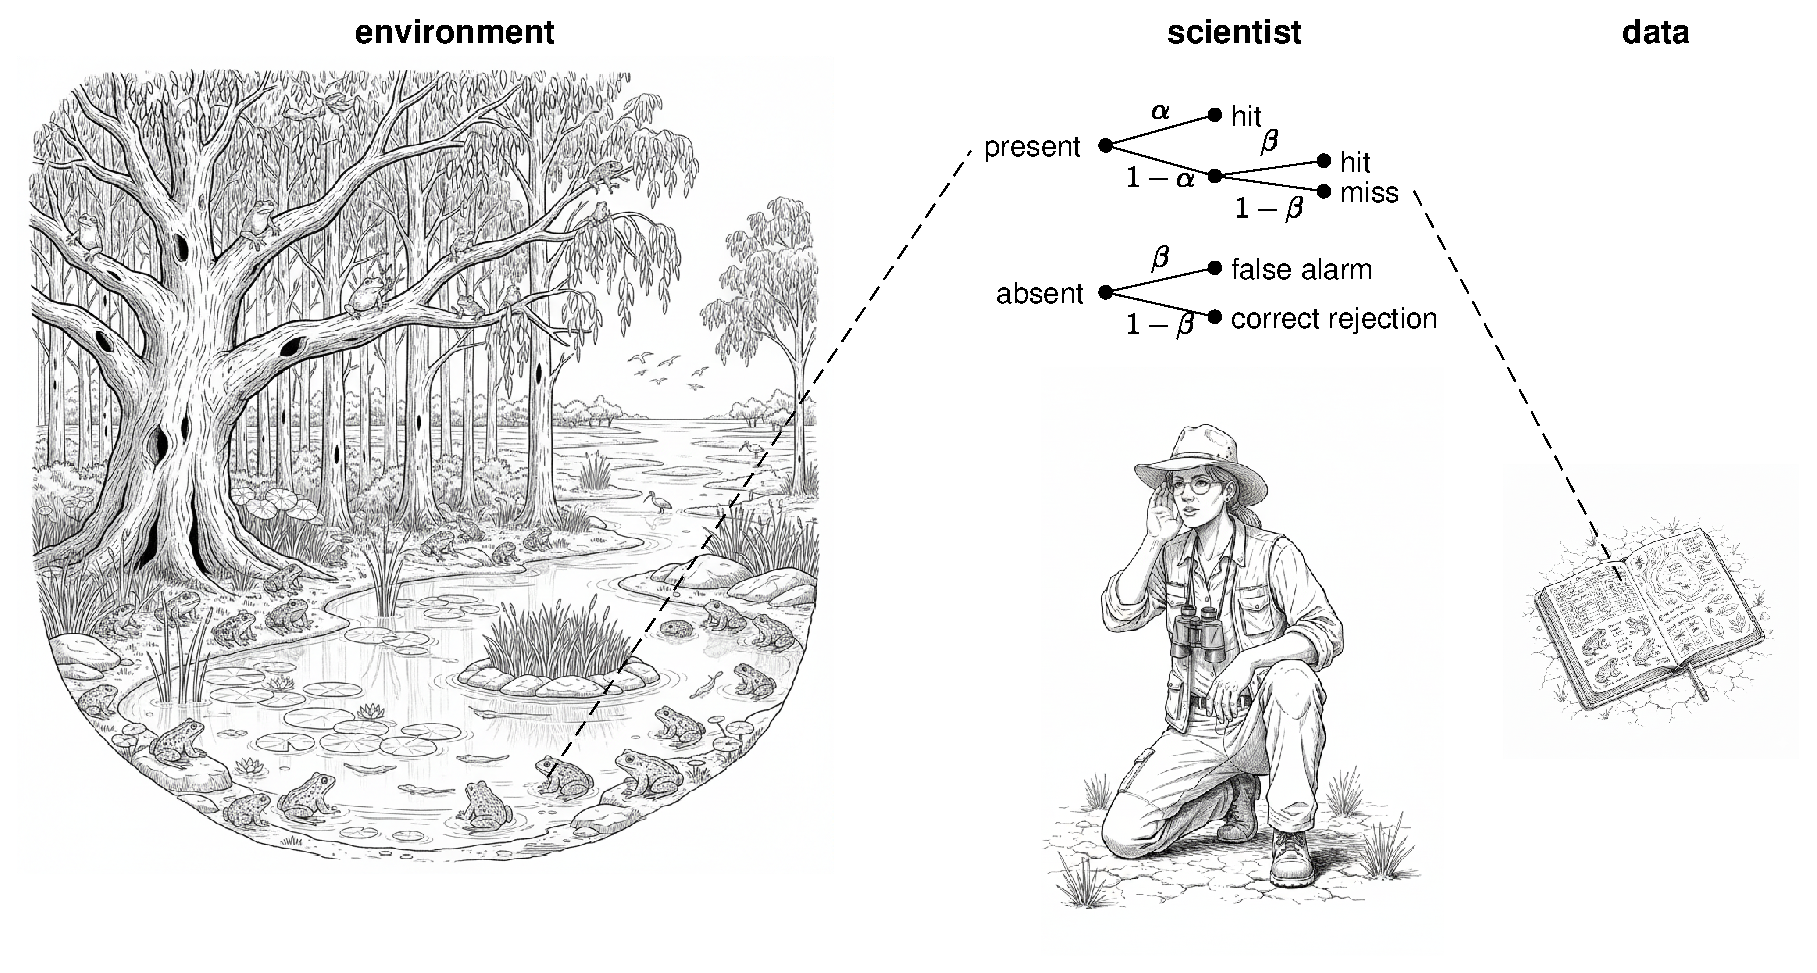
\includegraphics[width = \columnwidth, trim = {0cm 0cm 0cm 0cm}, clip]{../analyses/figures/frogPond.eps}\\
\end{center}
\end{frame}

\begin{frame}[fragile]{Model}
\vspace{-1em}
\bi
\i The model assumes frog $f$ in clip $j$ is either $\tau_{fj}=1$ present or $\tau_{fj}=1$ absent with a base-rate that depends on the frog $\psi_f$
\begin{eqnarray}
\tau_{fj} &\sim& \operatorname{Bernoulli}\bigl(\phi_j\bigr) \nonumber\\
\phi_j &\sim& \operatorname{Uniform}\bigl(0, 1\bigr) \nonumber
\end{eqnarray}
\i Individual $i$ judges frog $f$ in clip $j$ to be $y_{ijf}=1$ present with probability $\theta_{ijf}$ given by the one-high threshold model
\begin{eqnarray}
\alpha_i, \beta_i  &\sim & \operatorname{Uniform}\bigl(0, 1\bigr) \nonumber\\
\theta_{ijf} & = & \begin{cases}
\alpha_i+\left(1-\alpha_i\right)\beta_i & \mathrm{if}\ \tau_{fj}=1\\
\beta_i & \mathrm{if}\ \tau_{fj}=0
\end{cases}\nonumber\\
y_{ij} & \sim & \operatorname{Bernoulli}\bigl(\theta_{ij}\bigr)\nonumber
\end{eqnarray}
\i Implemented the model in JAGS and Stan
\ei
\end{frame}


\begin{frame}[fragile]{Model-Based Crowd Performance}
\vspace{-1em}
\bi
\i The performance of the model closely matches the results for the \citeA{brown2024cognitive} model
\bi
\j both model-based approaches improve on the tallying judgements
\ei
\ei
\begin{center}
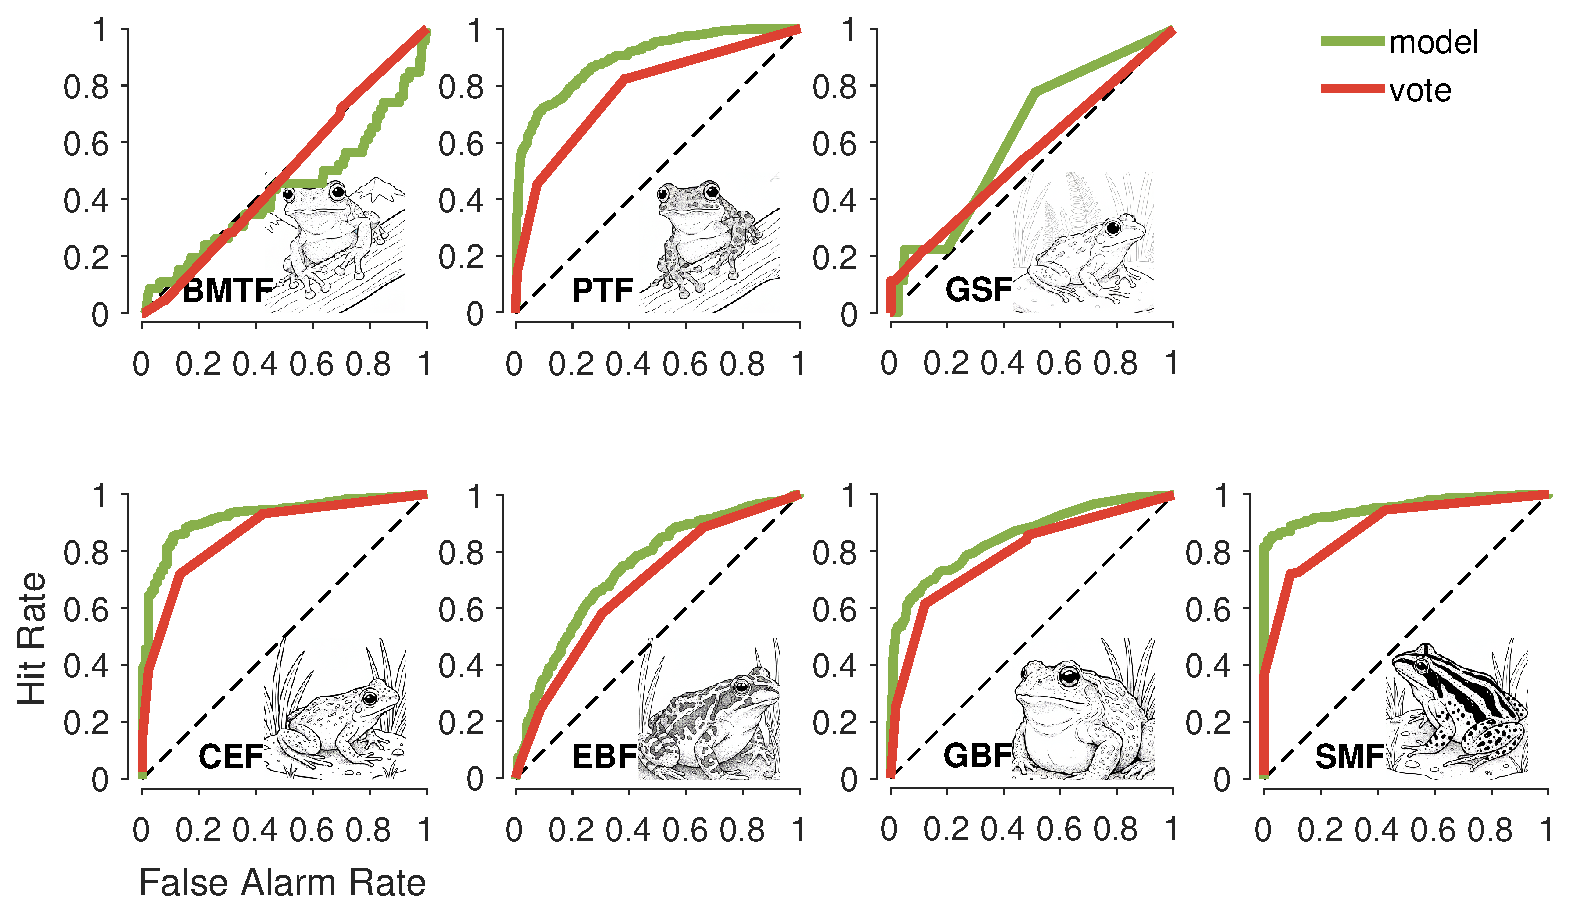
\includegraphics[width = \columnwidth, trim = {0cm 0cm 0cm 0cm}, clip]{../models/figures/jags_oneHighThresholdNoDifferences_n_citizenFrogsAll_ROCs.eps}\\
\end{center}
\end{frame}

\begin{frame}[fragile]{Inferences about Detection and Guessing Bias}
\vspace{-1em}
\bi
\i Inferences about detection ability $\alpha_i$ and guessing bias $\beta_i$ provide some \emph{prediction} about the performance of individual $i$
\bi
\j this allows, for example, ``yes'' judgments from non-experts to be explained away as guessing
\ei
\ei
\begin{center}
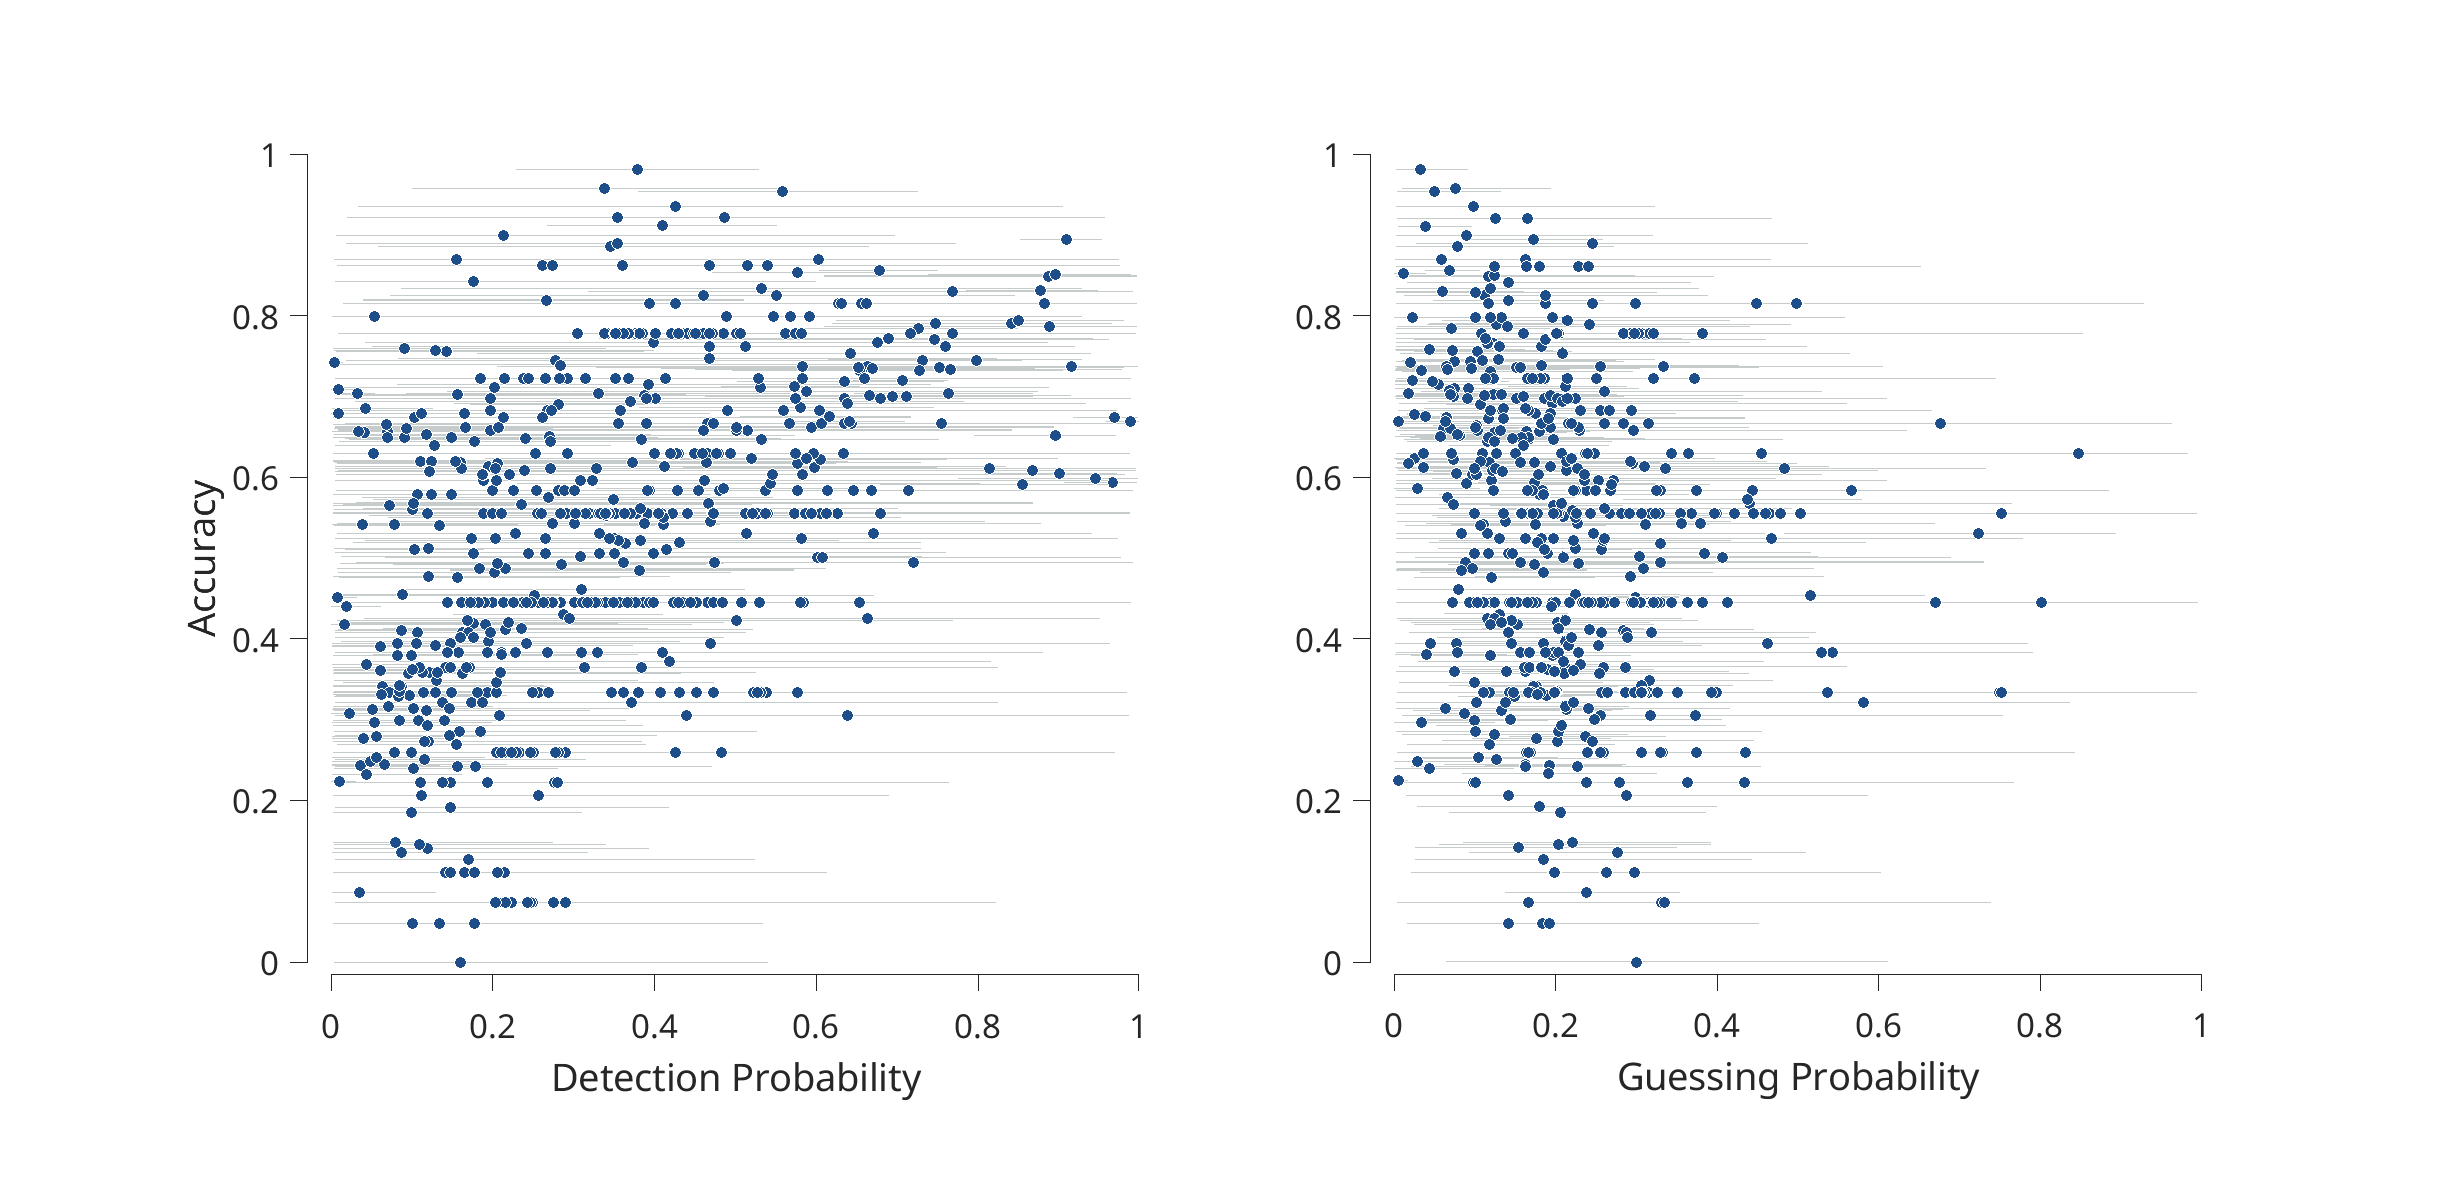
\includegraphics[width = \columnwidth, trim = {0cm 0cm 0cm 0cm}, clip]{../models/figures/jags_oneHighThresholdNoDifferences_n_citizenFrogsAll_parameters.eps}\\
\end{center}
\end{frame}


\begin{frame}[fragile]{Model-Based Crowd and the Truth}
\vspace{-1em}
\bi
\i \shortciteA{brown2024cognitive} point out that their model-based approach assumes independence over both scientists and clips
\bi
\j reasonable assumption for scientists, but there are obvious environmental dynamics that create dependencies over clips
\j ``frogs come and frogs go'' \textellipsis
\ei
\ei 
\begin{center}
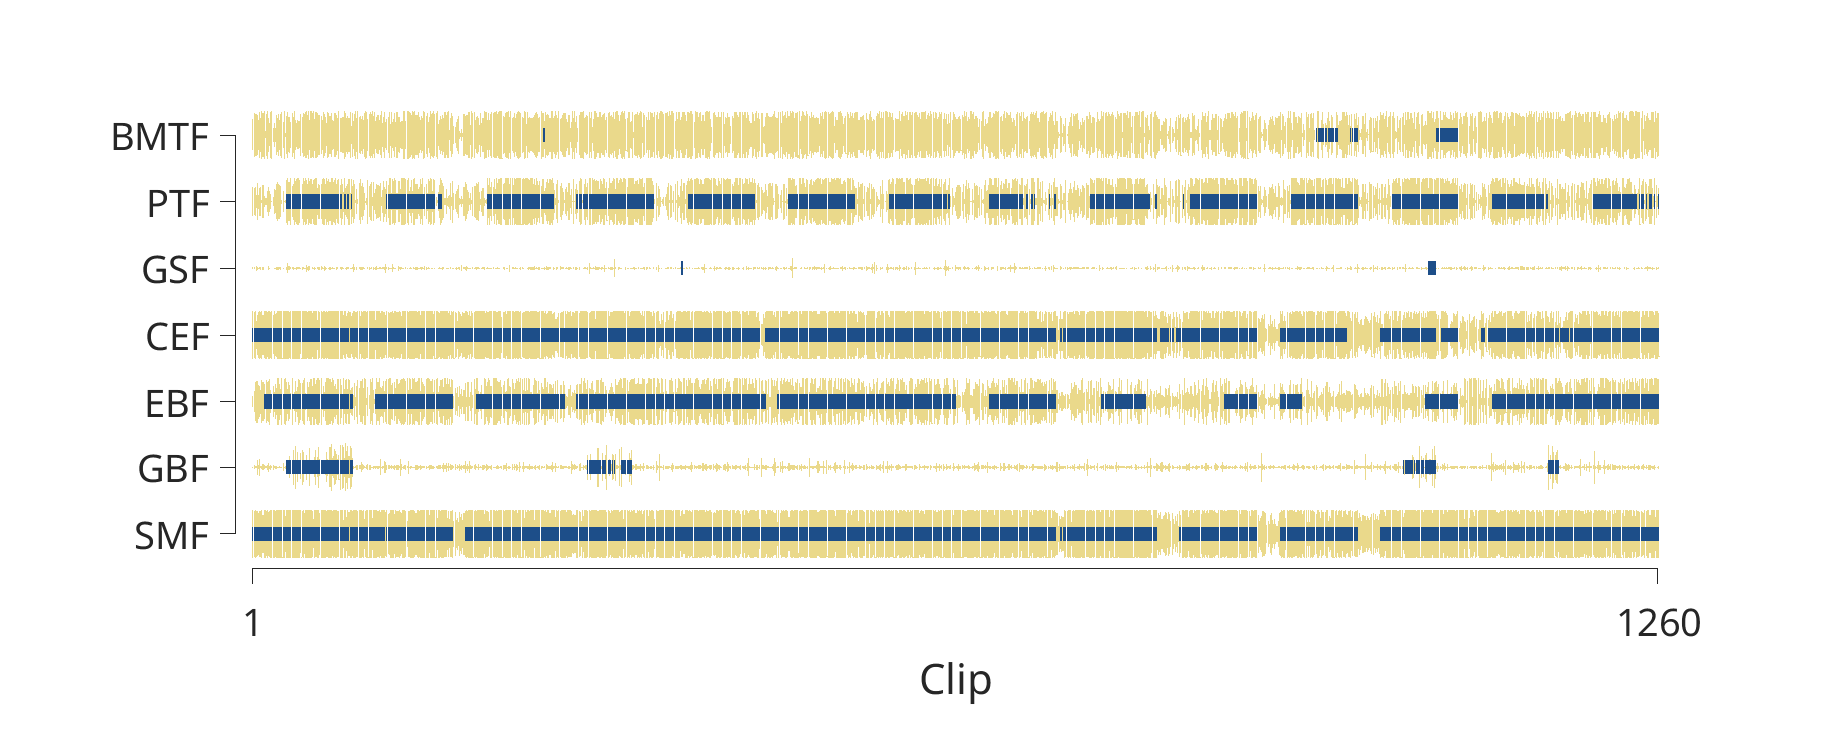
\includegraphics[width = \columnwidth, trim = {0cm 0cm 0cm 0cm}, clip]{../models/figures/jags_oneHighThresholdNoDifferences_n_citizenFrogsAll_environmentDynamics.eps}\\
\end{center}
\end{frame}


\begin{frame}[fragile]{Environment Dynamics Model and the Truth}
\vspace{-1em}
\bi 
\i The environmental model has a switching probability $\gamma_f$ for frog $f$
\begin{eqnarray}
\gamma_f & \sim & \operatorname{Uniform}\bigl(0, 1\bigr) \nonumber \\
\tau_{f1} &\sim& \operatorname{Bernoulli}\bigl(\frac{1}{2}\bigr) \nonumber\\
\tau_{fk} & \sim& \begin{cases}
\operatorname{Bernoulli}\bigl(\gamma_f \bigr) & \mathrm{if}\ \tau_{f\left(k-1\right)}=1\\
\operatorname{Bernoulli}\bigl(1-\gamma_f \bigr) & \mathrm{if}\ \tau_{f\left(k-1\right)}=0,\ k>1
\end{cases} \nonumber
\end{eqnarray}
\ei
\begin{center}
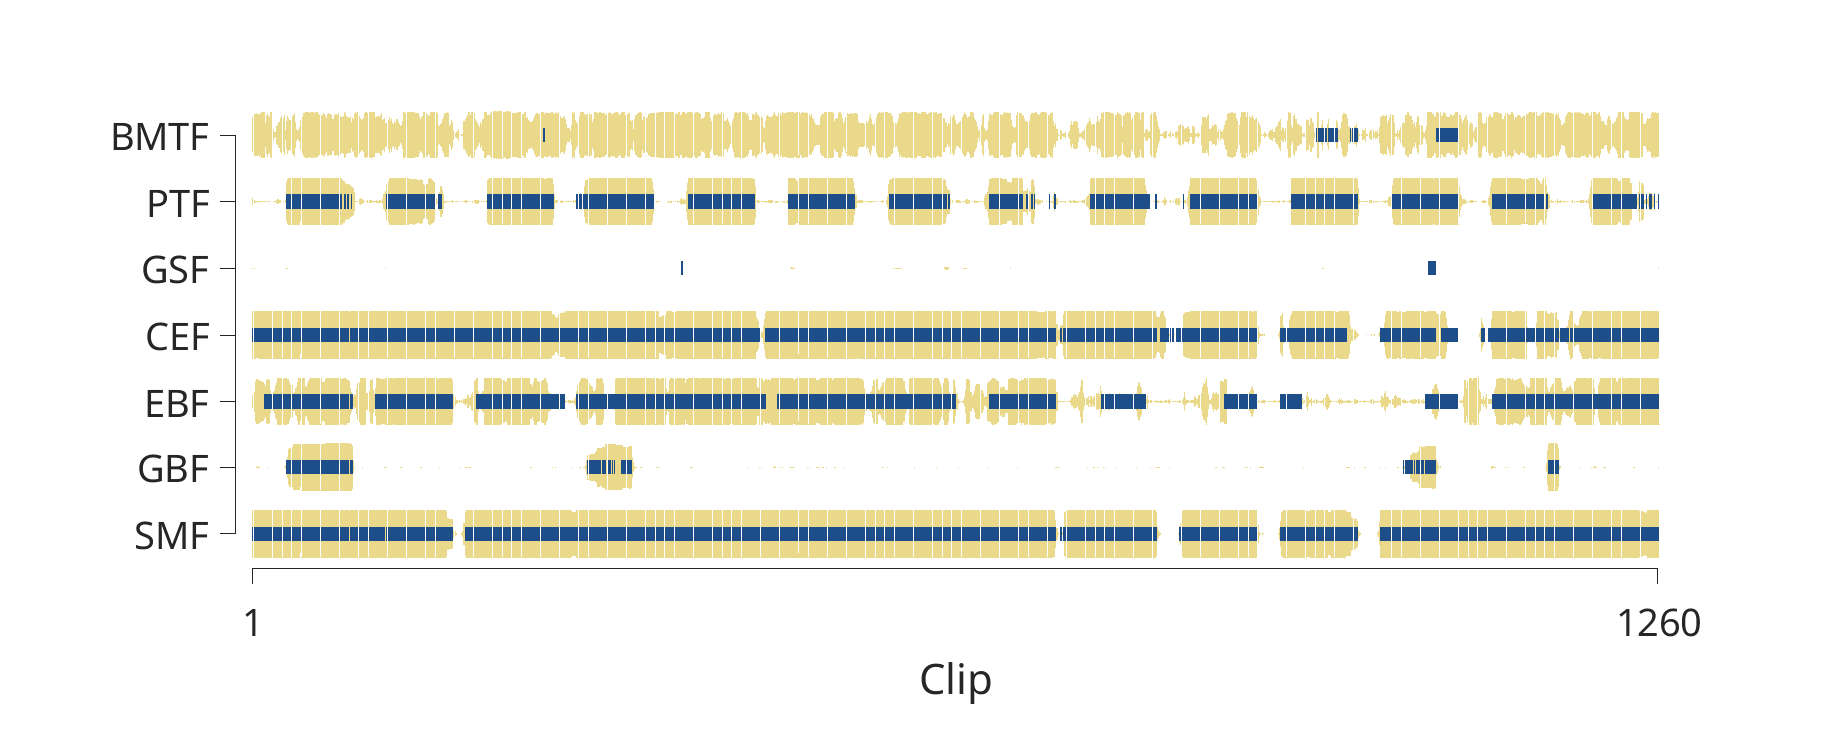
\includegraphics[width = \columnwidth, trim = {0cm 0cm 0cm 0cm}, clip]{../models/figures/jags_oneHighThresholdNoDifferencesDynamics_n_citizenFrogsAll_environmentDynamics.eps}\\
\end{center}
\end{frame}

\begin{frame}[fragile]{Environment Dynamics Model Performance}
\vspace{-1em}
\begin{center}
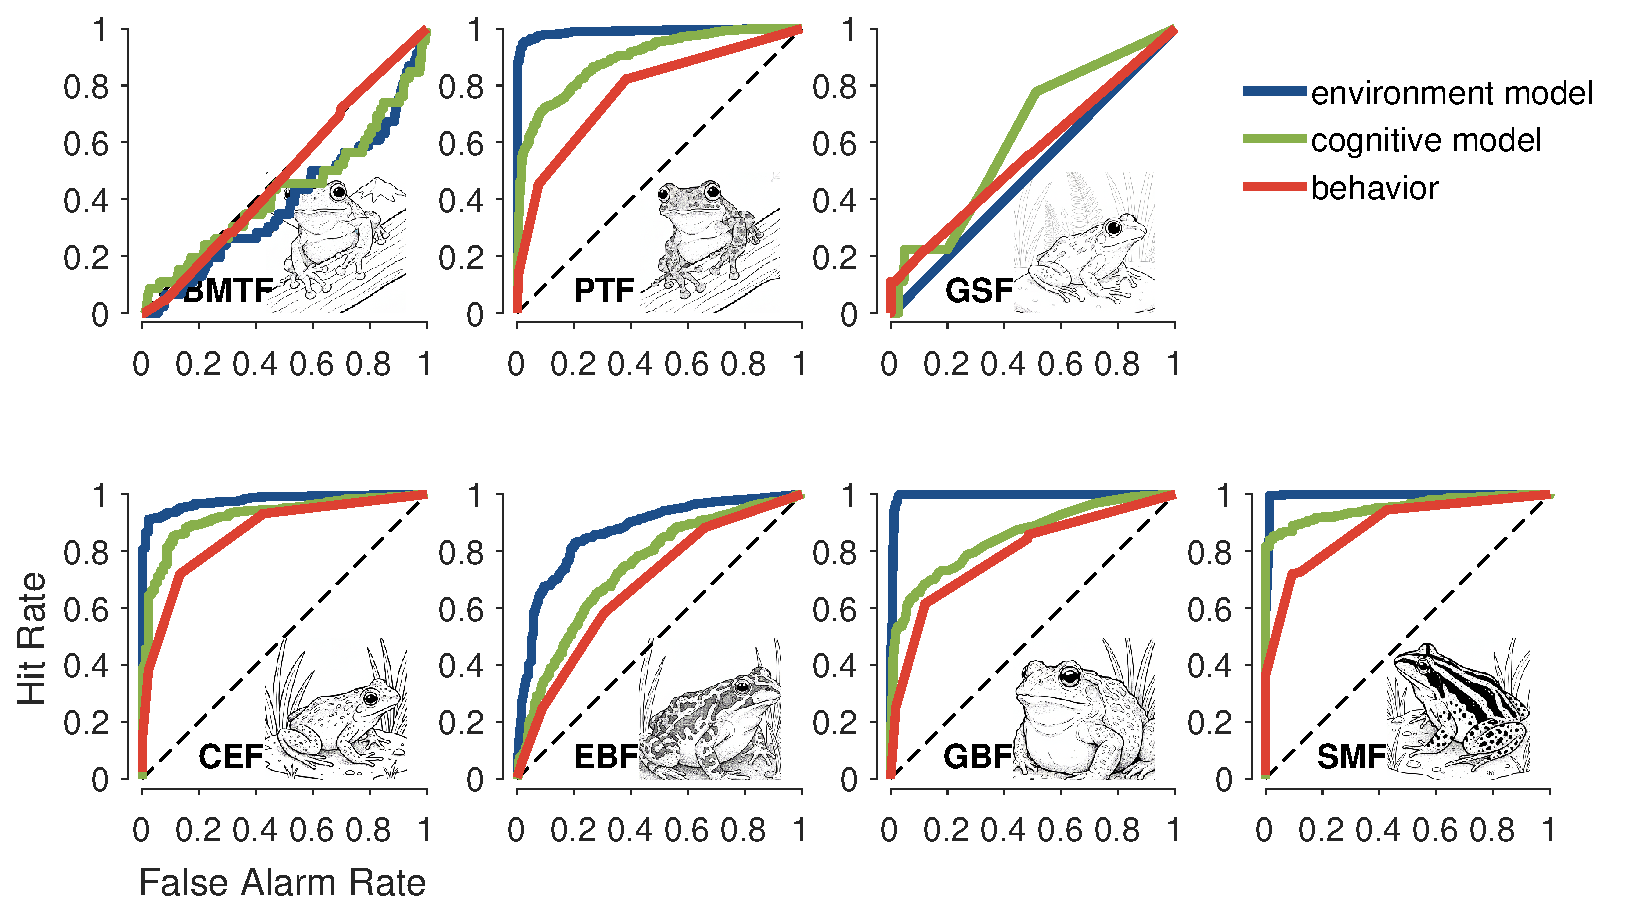
\includegraphics[width = \columnwidth, trim = {0cm 0cm 0cm 0cm}, clip]{../models/figures/jags_oneHighThresholdNoDifferencesDynamics_n_citizenFrogsAll_ROCs.eps}\\
\end{center}
\end{frame}


\begin{frame}[allowframebreaks]{References}
\bibliographystyle{apacite}
\bibliography{citizenFrogs}
\end{frame}


\begin{frame}[fragile]{\protect\shortciteA{brown2024cognitive} Model}
\vspace{-1em}
\begin{center}
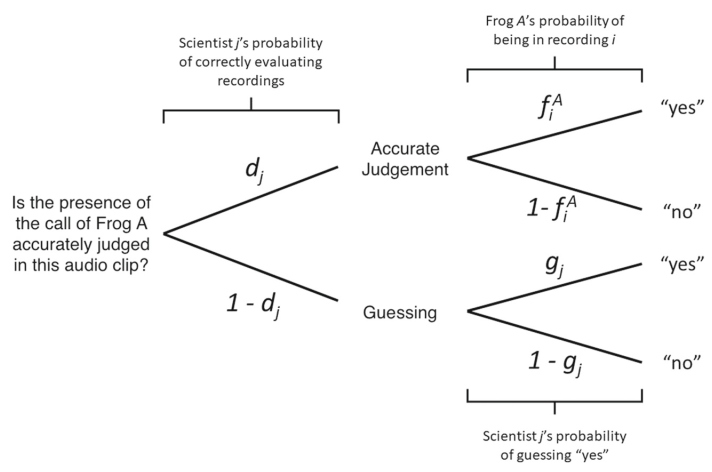
\includegraphics[width = \columnwidth, trim = {0cm 0cm 0cm 0cm}, clip]{../analyses/figures/brownModel.png}\\,
\end{center}
\end{frame}

\begin{frame}[fragile]{\protect\shortciteA{brown2024cognitive} Results}
\vspace{-1em}
\begin{center}
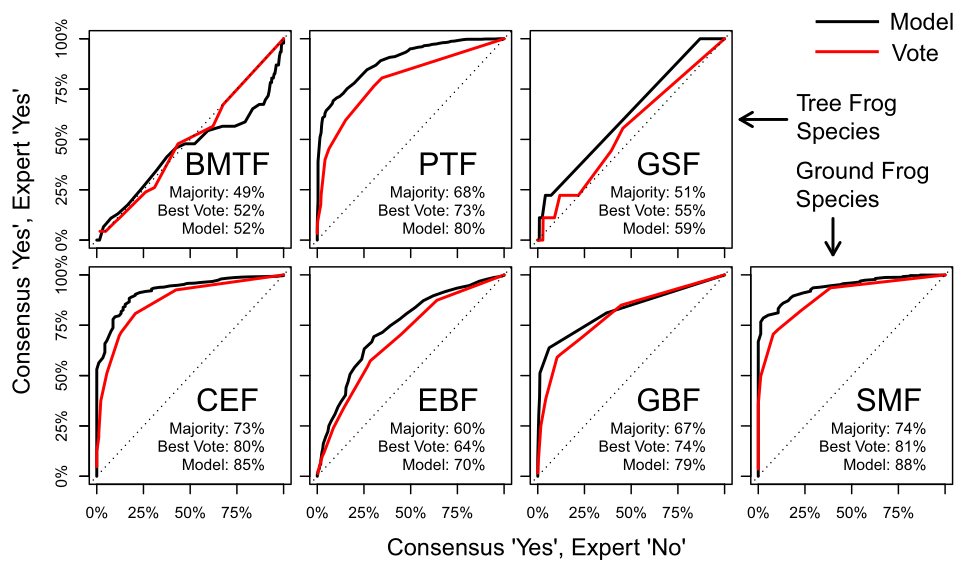
\includegraphics[width = \columnwidth, trim = {0cm 0cm 0cm 0cm}, clip]{../analyses/figures/brownResults.png}\\
\end{center}
\end{frame}

\end{document}
